\section{Monocular SLAM}
    \begin{frame}{Monocular SLAM}
        \textbf{PTAM}
        \vspace{-0.5cm}
        \fig{0.6}{ptamtracking}
        %~ {\tiny\href{http://www.youtube.com/watch?feature=player_embedded&v=Y9HMn6bd-v8}{[YouTube]}}
        \vspace{-0.7cm}
        \begin{itemize}
            \item Measurements are not metric.
            %~ \item A similar library, SceneLib, provides this.
        \end{itemize}
    \end{frame}
    \note{
        For the video based SLAM part of this thesis, a library called PTAM was used.
        Again, the idea is to track features, here shown as dots, through
        the video frames to estimate the camera's position.
        One major problem with video based tracking is that, unless you know something
        about the recorded scene, there is no way of knowing wether its a large scene
        that moved a lot, or a small scene that just moved a little.
        As for instance when you film a doll house, there is simply no way
        to tell it from a real house, and yet the scale of movement is completely different.

        The scaling needs to be extracted from other sources, and autonomously so since
        the PTAM coordinate system is initialized quite arbitrarily.
        This coordinate system is of central importance, since all measurements
        are given relative to it, and yet both orientation, position and scale is initially unknown.
    }
    \begin{frame}{Camera Measurements}
        \textbf{Measurement: } Pose relative to PTAM coordinate system.
        \vspace{-0.4cm}
        \begin{figure}[H]
        \centering
            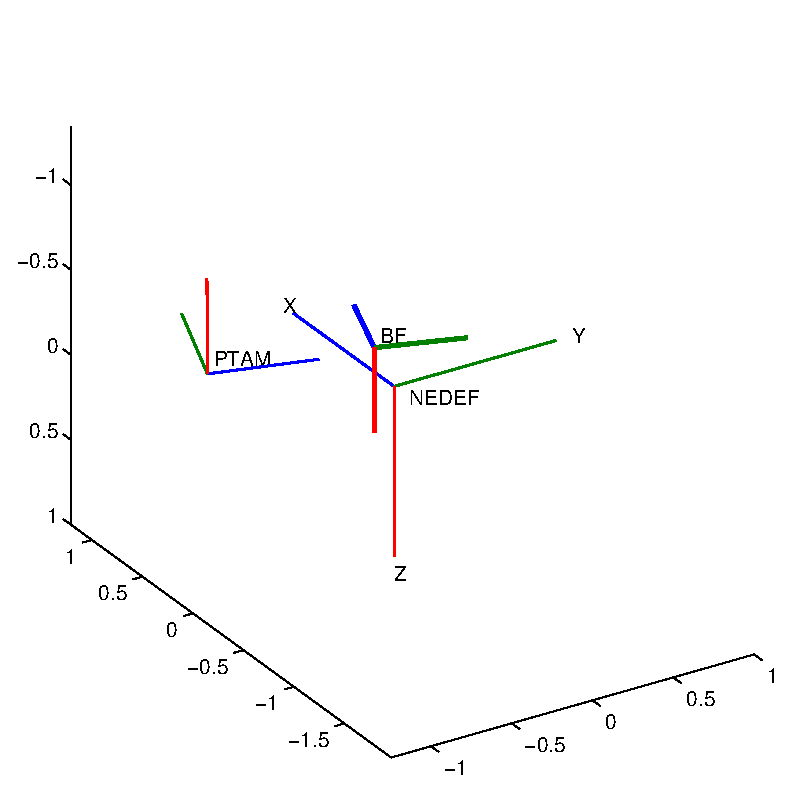
\includegraphics[trim = 0mm 0mm 0mm 20mm,clip,width=0.5\textwidth]{\currentchapter/figures/worldcoordframes}
        \end{figure}

        \vspace{-1cm}
        %~ The PTAM library is intended for use in Augmented Reality, AR.
        \begin{itemize}
            \item Rotation and translation are measured in the local PTAM coordinate system.
            \item PTAM's coordinate system is quite arbitrarily initialised.
            \item Its relation to the world must be established.
        \end{itemize}
        %~ \begin{itemize}
            %~ \item Intended to be used with wide-angle lens.
        %~ \end{itemize}
     % Intended for AR applications.
     % Intended for use with wide-angle camera lenses
    \end{frame}
    \note{}


    \subsection{Initialization}
    \begin{frame}{Initialization}
        PTAM tries to initialize its coordinate system on ground plane.
        %~ \vspace{-2cm}
        %~ \fig{0.7}{ground}
        \vspace{-0.5cm}
        \begin{figure}[h]
        \centering
            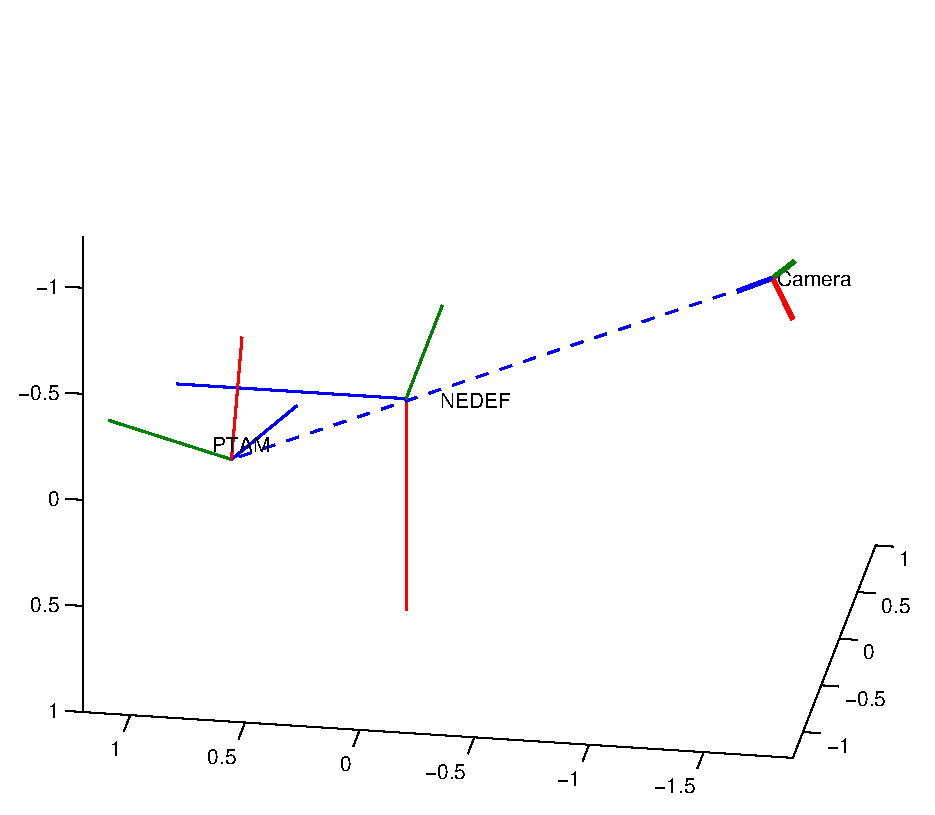
\includegraphics[trim = 0mm 0mm 0mm 20mm,clip,width=0.6\textwidth]{\currentchapter/figures/ground}
        \end{figure}

        \vspace{-1cm}
        \begin{align*}
            \left\lbrace
            \begin{array}{ll}
                \varnothing_{\text{PTAM}} &= \xi + R(q^{wb}) r_{\text{camera}/\mathcal{G}} + \lambda R(q^{wP}) \frac{X^{PTAM}}{|X^{PTAM}|} \\
                \varnothing_{\text{PTAM}} \cdot \hat{z} &= 0
            \end{array}\right. \\
        \end{align*}
        %~ \begin{equation*}
            %~ s = \frac{|X^{PTAM}|}{|\lambda|}
        %~ \end{equation*}
    \end{frame}

    \subsection{Connecting the Coordinate Systems}
    \begin{frame}{Camera Measurements}
        To extract positioning measurements usable in the real world,
        the coordinate systems have to be related.
        \begin{align*}
            x^{\text{PTAM}} &= S(s) R(q^{Pw}) T(-\varnothing_{\text{PTAM}}) x^{\text{NEDEF}} \\
            q^{Pw} &= q^{PTAM,c} q^{cb} q^{bw}
        \end{align*}
\vspace{-1cm}
        \begin{itemize}
            \item Describes the measurements in terms of the estimated state and known transformations.
            %~ \item Measurement equation for the state estimation.
        \end{itemize}
\vspace{-0.5cm}
        \begin{figure}[h]
        \centering
            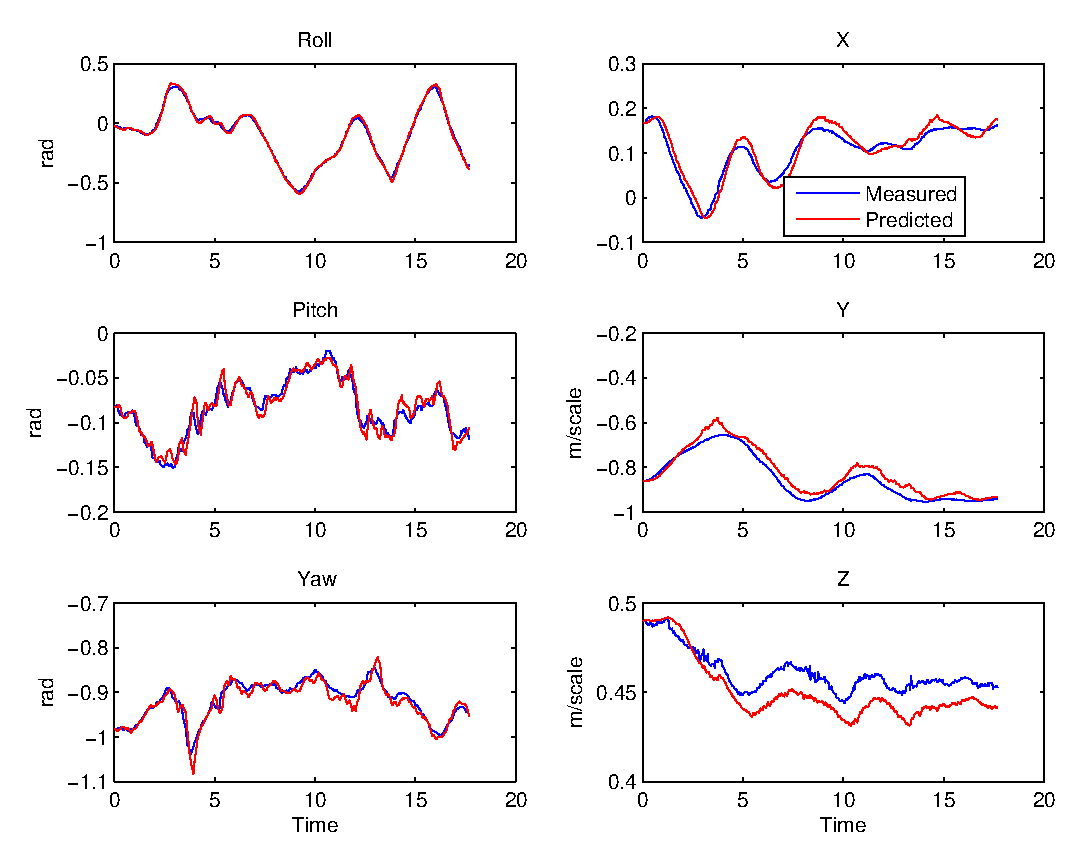
\includegraphics[trim = 0mm 50mm 0mm 0mm,clip,width=0.6\textwidth]{\currentchapter/figures/camera}
        \end{figure}

    \end{frame}

    \subsection{Library Modifications}
    \begin{frame}{Library Modifications}
        In a deployment environment, the initialization and utilization of
        the camera sensor must be autonomous.

        In the thesis, several changes are implemented to the PTAM library, e.g.
        \begin{itemize}
            \item Autonomous initialization procedure,
            \item Re-initialization,
            \item Origin positioning error detection,
            \item Remote interface for non-GUI use.
        \end{itemize}
    \end{frame}
